% Shared body of the paper. Included by main.tex (single author) and by local
% wrappers with a different author block. Do not put author information here.

\begin{abstract}
\noindent
We study the correlation risk premium on the S\&P~500 and the dispersion trade that harvests it, using OptionMetrics IvyDB US and CRSP data from January 1996 to August 2025. Implied correlation exceeds subsequently realized correlation in 80\% of months at the three-month horizon, by 8.5 correlation points on average ($t = 8.4$). A monthly ladder of vega-neutral, delta-hedged straddle dispersion tranches (short SPX, long the 50 largest members) earns 1.88 vol points per tranche before costs and 0.97 after half-spreads measured on listed options (annualized Sharpe ratio 0.56). The return is not explained by the market, Fama--French five factors, momentum or changes in VIX, and it is essentially uncorrelated with a short position in index volatility; its market beta is negative. The edge, however, is concentrated in 1996--2007 and in crisis periods, is not significant in 2010--2019, and vanishes at about twice the measured transaction costs. We then pre-register a conditional version of the trade, which opens a tranche only when implied correlation is rich relative to a HAR forecast of realized correlation, net of costs, and the volatility regime is calm. All parameters are estimated on 1996--2010 and frozen; the rule is tested once on 2011--2025 against a vega-matched unconditional benchmark.
\end{abstract}

\vspace{0.5em}
\noindent\textbf{Status of this draft.} Sections~\ref{sec:premium} and~\ref{sec:standard} are complete. Section~\ref{sec:conditional} reports the pre-registered design and every quantity estimated on the estimation sample; its out-of-sample results are deliberately not yet computed. Section~\ref{sec:final} will describe the final trade, which is designed and pre-registered before the test of Section~\ref{sec:conditional} is run.

\section{Introduction}

The variance of an index is the sum of its members' variances and covariances. Options on the index therefore price, besides the volatility of each member, the average correlation among them. \citet{DMV2009} show that index options are expensive relative to their constituents: the correlation implied by option prices exceeds the correlation subsequently realized, and the gap compensates investors for bearing correlation risk, which rises precisely when diversification fails. The trade that harvests this gap is the \emph{dispersion trade}: sell index volatility, buy constituent volatility. \citet{Marshall2009} documents its profitability on U.S.\ options.

This paper asks three questions, all on the S\&P~500 over 1996--2025.
\begin{enumerate}
  \item How large and how stable is the correlation risk premium? (Section~\ref{sec:premium})
  \item Does a realistic dispersion trade earn it after transaction costs, and is the return compensation for exposure to standard risk factors? (Section~\ref{sec:standard})
  \item Can timing the trade, opening it only when the premium is large relative to costs and to a forecast of realized correlation, improve its risk-adjusted return and limit its drawdowns? (Sections~\ref{sec:conditional} and~\ref{sec:final})
\end{enumerate}

Two features distinguish our approach. First, all trade P\&L is computed on actual price paths with exact daily delta hedging, and costs are measured on the listed contracts that would have been traded, rather than approximated by ``vega times realized minus implied volatility'' with assumed spreads. The approximation matters: its correlation with the exact P\&L is only 0.64. Second, the conditional trade is \emph{pre-registered}. Its data, definitions, trading rule, the way each parameter is chosen and the criteria that decide whether it is kept or dropped were committed to a public repository before any signal or P\&L was computed. Parameters are estimated on 1996--2010 and frozen; 2011--2025 is used once.

All code is public.\footnote{\url{https://github.com/LucaDennert/conditional-dispersion-sp500}. The licensed data are not redistributed; the repository contains the extraction queries, the code and the aggregated results.}

\section{Data and definitions}\label{sec:data}

\paragraph{Sources.} Option data come from OptionMetrics IvyDB US (via WRDS): standardized options (91- and 30-day ATM-forward implied volatilities, \texttt{stdopd}), the 91-day volatility surface on a delta grid (\texttt{vsurfd}), listed option prices with bid, ask and greeks (\texttt{opprcd}), security prices (\texttt{secprd}) and the zero-coupon curve (\texttt{zerocd}). S\&P~500 membership, market capitalization and daily returns come from CRSP; members are linked to OptionMetrics through the WRDS link table (score~1). Fama--French factors and momentum come from WRDS. The sample runs from 4~January 1996 to 29~August 2025.

\paragraph{Dates and weights.} Signals are computed and trades opened on the first trading day of each month. The weight $w_i$ of member $i$ is its CRSP market capitalization at the previous month end divided by the total over members with valid data.

\paragraph{Implied and realized correlation.} With index volatility $\sigma_I$ and member volatilities $\sigma_i$, the average correlation $\rho$ is the single pairwise correlation that reproduces the index variance:
\begin{equation}\label{eq:avgcorr}
  \sigma_I^2 = \sum_i w_i^2\sigma_i^2 + \rho\sum_{i\neq j} w_i w_j \sigma_i\sigma_j
  \quad\Longrightarrow\quad
  \rho = \frac{\sigma_I^2 - \sum_i w_i^2\sigma_i^2}{\bigl(\sum_i w_i\sigma_i\bigr)^2 - \sum_i w_i^2\sigma_i^2}.
\end{equation}
\emph{Implied correlation} (IC) uses ATM-forward implied volatilities of the index and of all members; \emph{realized correlation} (RC) uses annualized realized volatilities of daily log returns. We write IC$_h$ for maturity $h$ (30 or 91 days) and RC$_n$ for a window of $n$ trading days.

\section{The correlation risk premium, 1996--2025}\label{sec:premium}

We compare implied correlation on each entry date with the correlation realized over the life of the options: IC$_{91}$ against RC over the following 63 trading days, and IC$_{30}$ against RC over the following 21 days. Figure~\ref{fig:premium} shows the two series and Table~\ref{tab:premium} summarizes them.

\begin{figure}[t]
  \centering
  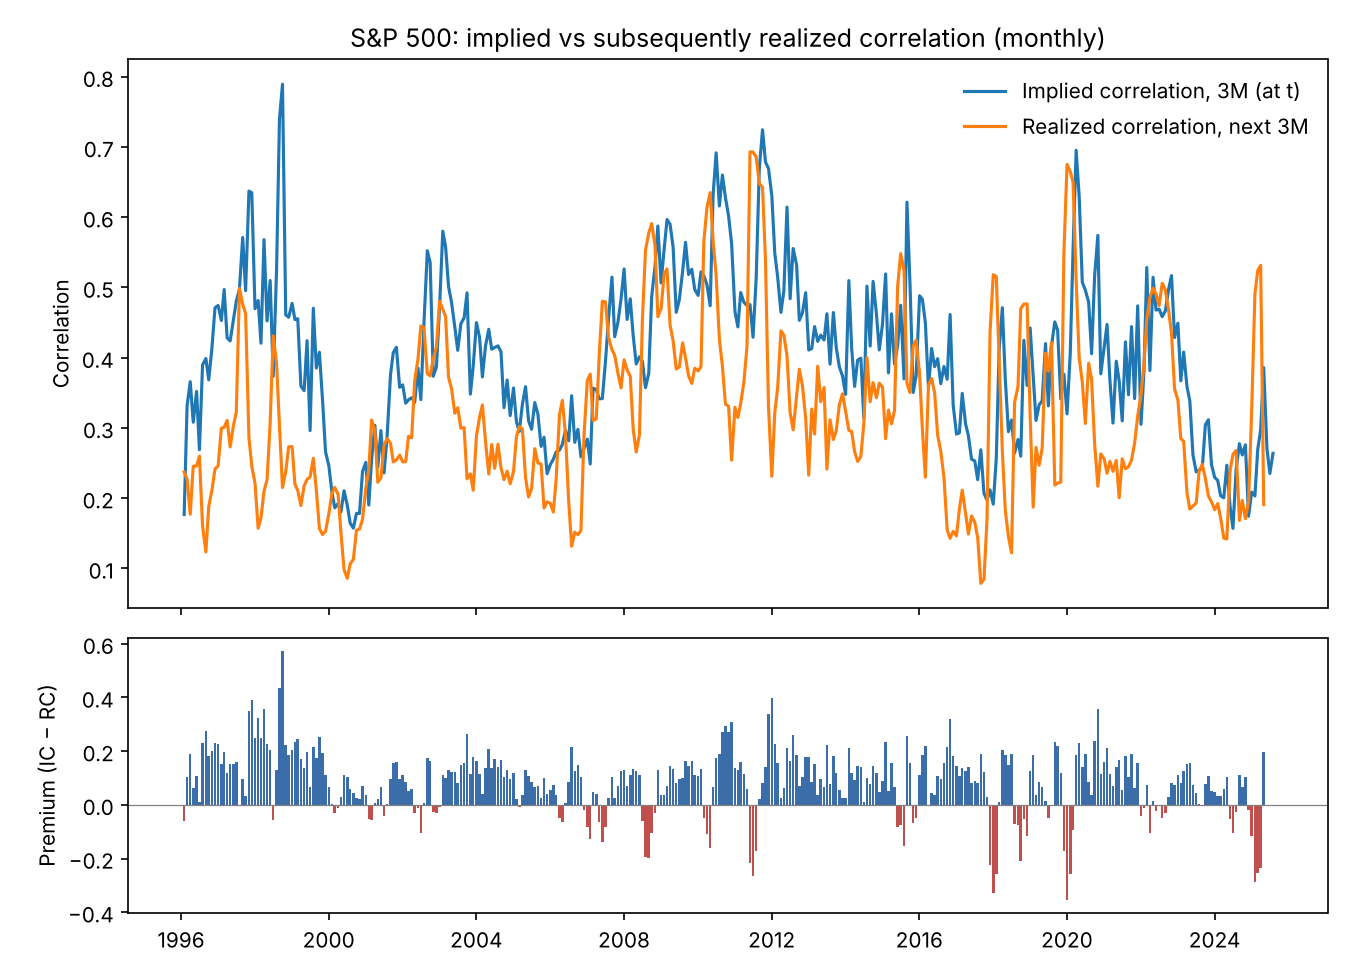
\includegraphics[width=\textwidth]{figures/fig_correlation_premium.png}
  \caption{Three-month implied correlation of the S\&P~500 and the correlation realized over the following three months (top), and their difference (bottom). Monthly, January 1996 to August 2025.}
  \label{fig:premium}
\end{figure}

\begin{table}[t]
  \centering
  \caption{Correlation risk premium: implied correlation minus subsequently realized correlation. $t$-statistics use Newey--West standard errors.}
  \label{tab:premium}
  \begin{tabular}{llrrrrrr}
    \toprule
    Period & Maturity & Months & IC & RC (after) & Premium & $t$ & Share $>0$ \\
    \midrule
    1996--2007 & 1M & 143 & 0.352 & 0.275 & 0.076 & 7.05 & 77\% \\
               & 3M & 143 & 0.375 & 0.271 & 0.104 & 7.14 & 84\% \\
    2008--2009 & 1M &  24 & 0.481 & 0.431 & 0.050 & 2.00 & 79\% \\
               & 3M &  24 & 0.492 & 0.429 & 0.063 & 1.86 & 79\% \\
    2010--2019 & 1M & 120 & 0.377 & 0.335 & 0.042 & 3.05 & 68\% \\
               & 3M & 120 & 0.430 & 0.343 & 0.086 & 4.98 & 81\% \\
    2020--2025 & 1M &  67 & 0.326 & 0.309 & 0.016 & 0.96 & 55\% \\
               & 3M &  65 & 0.367 & 0.319 & 0.048 & 2.02 & 71\% \\
    \midrule
    Full sample & 1M & 354 & 0.364 & 0.313 & 0.051 & 6.84 & 70\% \\
                & 3M & 352 & 0.400 & 0.315 & 0.085 & 8.45 & 80\% \\
    \bottomrule
  \end{tabular}
\end{table}

\paragraph{Findings.}
\begin{itemize}
  \item \textbf{The premium is large and persistent.} At three months, implied correlation exceeds realized correlation by 8.5 points on average and in 80\% of months. It is positive and significant in every sub-period, although it has roughly halved since 2020.
  \item \textbf{It is larger at three months than at one.} The one-month premium is 5.1 points and is not significant in 2020--2025.
  \item \textbf{It is higher when volatility is higher.} Sorting months by VIX terciles, the three-month premium is 4.0 points in the low tercile and 10--11 points in the middle and high terciles. Regressing the premium on the level of implied correlation gives a slope of 0.51 ($t = 6.5$, $R^2 = 0.23$): when implied correlation is high, about half of it is premium.
\end{itemize}
The last point is the starting idea of the conditional trade: the premium is predictable, at least in part, from quantities observed on the trade date.

\section{The unconditional dispersion trade}\label{sec:standard}

\subsection{Construction}

On the first trading day of every month we open a three-month tranche:
\begin{itemize}
  \item \textbf{short} an ATM-forward straddle on SPX;
  \item \textbf{long} ATM-forward straddles on the 50 largest members, with vega allocated by index weight;
  \item \textbf{vega-neutral}: the two legs carry the same vega.
\end{itemize}
Each straddle is delta-hedged daily and held to expiry (63 trading days), so three tranches are live at any time. The trade is long the dispersion of member volatilities around the index: it gains when realized correlation is below the correlation priced into the index.

\paragraph{Exact P\&L.} Entry prices are Black--Scholes prices at the market implied volatility (91-day ATM-forward). The hedge and the payoff are computed on the actual price paths (CRSP for members, including dividends; SPX with dividends at the yield implied by the 91-day forward). With spot normalized to one, strike $K = e^{(r-q)T}$, and $V_t$, $\Delta_t$ the Black--Scholes straddle value and delta at the inception volatility, the P\&L of a long hedged straddle is
\begin{equation}\label{eq:pnl}
  \Pi = |S_T - K| - V_0 - \sum_{t=0}^{T-1}\Delta_t S_t R_{t+1} - \sum_{t=0}^{T-1} r\,(V_t - \Delta_t S_t)\,\delta t,
\end{equation}
where $R_{t+1}$ is the total return of the underlying and $r$ is the 91-day zero rate. We express $\Pi$ in vol points per unit of initial vega, so that legs are comparable and the tranche P\&L is $\sum_i \tilde w_i \Pi_i/\nu_i - \Pi_I/\nu_I$, with $\tilde w_i$ the weights renormalized within the basket. For a book with \$100{,}000 of vega per leg, one vol point is \$100{,}000 per tranche.

\paragraph{Measured costs.} On each entry date we select, for SPX and for each of the 50 names, the standard monthly listed straddle closest to 91 days and to the spot strike, with both legs quoted, choosing the tightest spread when several qualify. The half-spread in vol points is $(\text{spread}_C + \text{spread}_P)/2$ divided by the straddle vega. The basket cost is index-weighted; names with no listed quote on that date take the basket median. Since straddles are held to expiry, only the entry half-spread is paid. Table~\ref{tab:costs} reports the result.

\begin{table}[t]
  \centering
  \caption{Measured entry half-spreads of three-month near-ATM listed straddles, vol points per unit of vega. ``Coverage'' is the share of basket weight with a listed contract on the entry date.}
  \label{tab:costs}
  \begin{tabular}{lrrr}
    \toprule
    Period & Single-stock basket & SPX & Coverage \\
    \midrule
    1996--2000 & 1.15 & 0.42 & 68\% \\
    2001--2007 & 0.70 & 0.48 & 70\% \\
    2008--2009 & 0.64 & 0.65 & 70\% \\
    2010--2019 & 0.26 & 0.31 & 89\% \\
    2020--2025 & 0.37 & 0.06 & 98\% \\
    \bottomrule
  \end{tabular}
\end{table}

Spreads fell with decimalization (2001) and the penny pilot (from 2007). Coverage is lower before 2010 because many single-stock options were listed on quarterly cycles, so no standard expiry fell near three months.

\subsection{Performance}

\begin{table}[t]
  \centering
  \caption{Unconditional dispersion trade, top-50 basket, net of measured costs. P\&L in vol points per tranche. $t$-statistics are Newey--West; Sharpe ratios are annualized from non-overlapping tranches.}
  \label{tab:perf}
  \begin{tabular}{lrrrrrrr}
    \toprule
    Period & Tranches & Mean & $t$ & Sharpe & Hit rate & Worst & Best \\
    \midrule
    1996--2007 & 143 & 1.44 & 3.23 & 0.82 & 64\% & $-6.2$ & 11.2 \\
    2008--2009 &  24 & 0.59 & 0.40 & 0.19 & 54\% & $-10.7$ & 15.9 \\
    2010--2019 & 120 & 0.33 & 1.24 & 0.31 & 61\% & $-8.8$ & 7.5 \\
    2020--2025 &  65 & 1.27 & 1.90 & 0.68 & 57\% & $-4.2$ & 18.8 \\
    \midrule
    Full sample & 352 & 0.97 & 3.79 & 0.56 & 61\% & $-10.7$ & 18.8 \\
    \bottomrule
  \end{tabular}
\end{table}

\begin{figure}[t]
  \centering
  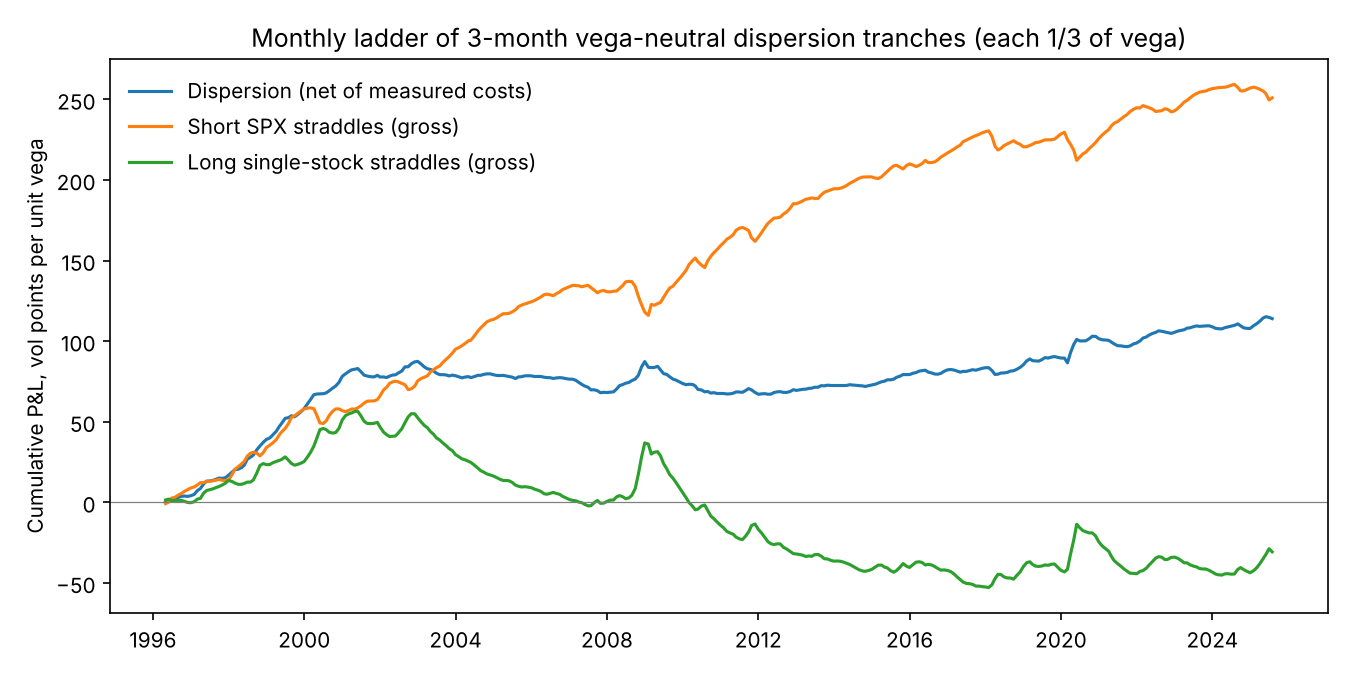
\includegraphics[width=0.9\textwidth]{figures/fig_simple_dispersion_cumulative.png}
  \caption{Cumulative P\&L of the monthly ladder (each tranche one-third of the vega budget): dispersion net of measured costs, and the two legs gross of costs.}
  \label{fig:cum}
\end{figure}

Table~\ref{tab:perf} and Figure~\ref{fig:cum} summarize the results.
\begin{itemize}
  \item \textbf{The trade is profitable after costs over the full sample}: 0.97 vol points per tranche ($t = 3.8$), Sharpe ratio 0.56. Gross of costs the mean is 1.88 and the Sharpe ratio 1.05. Using all members instead of the top 50 changes little (0.92, Sharpe 0.57).
  \item \textbf{The index leg earns the money.} Short SPX straddles earn $+2.14$ vol points per tranche, the index variance risk premium \citep{BakshiKapadia2003, CarrWu2009}. Long single-stock straddles lose $-0.26$, close to zero: single-stock implied volatility is approximately fair.
  \item \textbf{The edge is concentrated.} It comes from 1996--2007 and from the 2020s. In 2010--2019 the net mean is 0.33 vol points and not significant.
  \item \textbf{Costs are first order.} Break-even is at about twice the measured spreads (Table~\ref{tab:costsens}).
\end{itemize}

\begin{table}[t]
  \centering
  \caption{Sensitivity to transaction costs (top-50 basket, full sample). $1\times$ = measured half-spreads.}
  \label{tab:costsens}
  \begin{tabular}{lrrrrrr}
    \toprule
    Cost multiple & $0\times$ & $0.5\times$ & $1\times$ & $1.5\times$ & $2\times$ & $3\times$ \\
    \midrule
    Mean (vol pts) & 1.88 & 1.42 & 0.97 & 0.52 & 0.07 & $-0.84$ \\
    Sharpe         & 1.05 & 0.81 & 0.56 & 0.30 & 0.04 & $-0.47$ \\
    \bottomrule
  \end{tabular}
\end{table}

\subsection{Is it a risk-factor bet?}

We regress the net P\&L of each tranche on the factor returns summed over the tranche's life: the market, the five Fama--French factors \citep{FamaFrench2015}, momentum \citep{Carhart1997}, the change in VIX, and the P\&L of the short SPX straddle. Standard errors are Newey--West with two lags \citep{NeweyWest1987}, since consecutive tranches overlap.

\begin{table}[t]
  \centering
  \caption{Factor regressions of the net tranche P\&L (vol points). Factors are summed over each tranche's life (\%).}
  \label{tab:factors}
  \begin{tabular}{lrrr}
    \toprule
    Model & Alpha & $t$(alpha) & $R^2$ \\
    \midrule
    CAPM                         & 1.35 & 5.05 & 0.13 \\
    FF5 + momentum               & 1.36 & 4.82 & 0.20 \\
    FF5 + momentum + $\Delta$VIX & 1.30 & 4.82 & 0.20 \\
    Short SPX straddle only      & 1.13 & 3.22 & 0.01 \\
    All of the above             & 1.06 & 3.20 & 0.22 \\
    \bottomrule
  \end{tabular}
\end{table}

\begin{itemize}
  \item \textbf{Alpha survives every specification} (Table~\ref{tab:factors}), and standard factors explain at most a fifth of the variance.
  \item \textbf{Market beta is negative} ($-0.16$, $t = -4.3$ in the CAPM). A vega-neutral book is net long the \emph{level} of volatility, because single-stock volatilities move more in points than index volatility. This offsets the rise in correlation in sell-offs, which is why the 2008 and 2020 tranches were profitable.
  \item \textbf{It is not short index volatility in disguise}: the tranche P\&L is essentially uncorrelated with the short SPX straddle ($R^2 = 0.01$, Figure~\ref{fig:scatter}).
\end{itemize}

\begin{figure}[t]
  \centering
  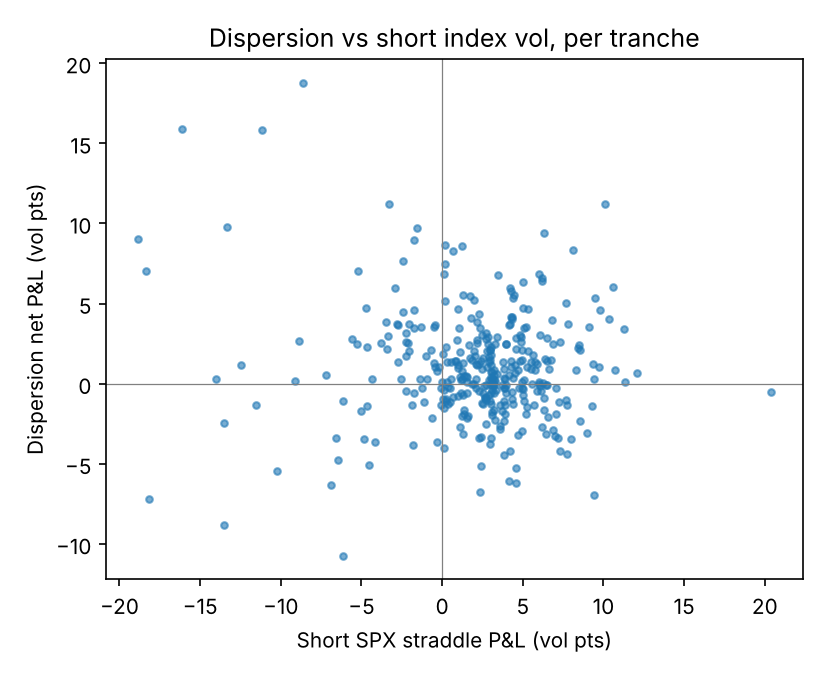
\includegraphics[width=0.55\textwidth]{figures/fig_dispersion_vs_short_vol.png}
  \caption{Dispersion P\&L against the P\&L of the short SPX straddle, per tranche.}
  \label{fig:scatter}
\end{figure}

\subsection{Straddles versus variance swaps}

The three-month model-free variance-swap strike of SPX \citep{BrittenJonesNeuberger2000}, computed from the IvyDB volatility surface in the same way as the VIX, averages 20.3 against 18.6 for ATM volatility. A short SPX variance swap struck at the model-free strike earns $+1.7$ vol points per tranche; struck at ATM volatility it would earn about zero. A variance-swap version of the dispersion trade therefore needs model-free strikes on both legs, which we compute from the member volatility surfaces in a robustness check. The straddle version is not affected, because straddles are priced at ATM volatility.

\subsection{Exact P\&L versus the usual approximation}

A common shortcut values a delta-hedged option as vega times realized minus implied volatility. Across our tranches its correlation with the exact P\&L of equation~\eqref{eq:pnl} is 0.64, with a mean gap of $-0.24$ vol points. Gamma is path dependent and concentrated near the strike, and large moves, which drive the dispersion P\&L, are where the shortcut fails.

\section{A pre-registered conditional dispersion trade}\label{sec:conditional}

\subsection{Hypothesis and protocol}

Section~\ref{sec:premium} shows that the correlation premium is predictable and Section~\ref{sec:standard} that the unconditional trade is thin after costs and loses in some regimes. \textbf{Hypothesis:} opening tranches only when implied correlation is rich relative to a forecast of realized correlation, net of costs, and when the volatility regime is calm, improves the risk-adjusted return and reduces drawdowns relative to opening every month.

The rule, its parameters and the kill test were committed to the repository on 12~November 2026, before any signal or P\&L was computed (\texttt{PREREGISTRATION.md}). The estimation sample is 1996--2010; the test sample, 2011--2025, is used once.

\subsection{Correlation forecast}

On each entry date $t$ we forecast the correlation realized over the next 53 trading days, the typical life of a tranche (63 days to expiry minus a 10-day exit buffer), with a HAR regression \citep{Corsi2009} in Fisher-$z$ space:
\begin{equation}\label{eq:har}
  z(\mathrm{RC}^{\mathrm{fwd}}_t) = a + b_1 z(\mathrm{RC}_{21,t}) + b_2 z(\mathrm{RC}_{63,t}) + b_3 z(\mathrm{RC}_{252,t}) + b_4 z(\mathrm{IC}_t) + \varepsilon_t, \qquad z(x) = \operatorname{atanh}(x).
\end{equation}
It is estimated by OLS on the 166 entry dates whose target window ends by December 2010 and then frozen.

\begin{table}[t]
  \centering
  \caption{HAR forecast of realized correlation, estimation sample (1996--2010). Newey--West standard errors with three lags.}
  \label{tab:har}
  \begin{tabular}{lrr}
    \toprule
    & Coefficient & $t$ \\
    \midrule
    Constant          & 0.090 & 3.09 \\
    $z$(RC$_{21}$)    & 0.226 & 2.36 \\
    $z$(RC$_{63}$)    & 0.129 & 1.00 \\
    $z$(RC$_{252}$)   & 0.307 & 2.06 \\
    $z$(IC)           & 0.036 & 0.30 \\
    \midrule
    $R^2$ ($z$ space) & \multicolumn{2}{r}{0.42} \\
    RMSE (correlation units) & \multicolumn{2}{r}{0.088} \\
    \bottomrule
  \end{tabular}
\end{table}

Realized correlation is persistent at the monthly and yearly horizons; once past realized correlation is known, implied correlation adds nothing to the forecast (Table~\ref{tab:har}). The forecast beats the naive alternatives on the estimation sample (RMSE 0.088 against 0.115 for RC$_{21}$ and 0.103 for RC$_{63}$). The correlation premium used by the rule is $\mathrm{CP}_t = \mathrm{IC}_t - \widehat{\mathrm{RC}}_t$.

\subsection{Trading rule}

Open a tranche on entry date $t$ if and only if
\begin{equation}\label{eq:rule}
  \mathrm{CP}_t > c + k\cdot\mathrm{RMSE} \qquad\text{and}\qquad \mathrm{VIX}_t < \mathrm{VIX}^{(80)}_{1996\text{--}2010},
\end{equation}
with $k = 0.5$ and the VIX threshold equal to the 80th percentile of VIX closes in the estimation sample (26.8).

\paragraph{Cost threshold.} $c$ is the average round-trip cost of a tranche in correlation units, measured on the contracts actually selected. Per unit of tranche vega,
\[
  \text{cost}_t = h_{\mathrm{SPX}} + \sum_i \tilde w_i h_i, \qquad h_x = \frac{\text{half-spread at entry} + \text{half-spread at exit}}{\text{straddle vega at entry}},
\]
with the exit quote taken 10 trading days before expiry. From equation~\eqref{eq:avgcorr}, a change $d\rho$ in the correlation priced into the index moves index volatility by $d\sigma_I = C\,d\rho/(2\sigma_I)$, where $C = (\sum w_i\sigma_i)^2 - \sum w_i^2\sigma_i^2$. Since a vega-neutral tranche earns the index-volatility mispricing per unit of vega, the premium needed to pay the costs is $c_t = (\text{cost}_t/100)\cdot 2\sigma_I/C$. Averaging over 176 estimation-sample entry dates gives
\[
  c = 0.094 \quad\text{(round-trip cost 2.25 vol points: 0.80 SPX, 1.45 basket).}
\]
The rule therefore requires a premium of $0.094 + 0.5\times 0.088 = 0.138$. On the estimation sample this condition alone holds in 45 of 168 months (27\%).

\subsection{Trade construction and evaluation}

Contracts, sizing and execution follow the pre-registration. On each entry date, for SPX and for each of the top 50 members, we trade the standard monthly expiry closest to 91 days (60 to 130 days) and the strike closest to spot with both call and put quoted. The legs are vega-neutral, with the long-leg vega split by index weight. We buy at the ask and sell at the bid, hedge delta daily with IvyDB deltas (costs of 0.5\,bp of notional for the index and 1\,bp for stocks), keep at most three live tranches of one-third of the vega budget each, and exit 10 trading days before expiry. A missing quote is carried forward for at most three days.

The benchmark is the same ladder opening a tranche every month, rescaled to the same average vega as the conditional strategy. The strategy is \emph{kept} if, on 2011--2025,
\begin{enumerate}
  \item its Sharpe ratio exceeds the benchmark's with a one-sided block-bootstrap $p$-value below 0.10 (3-month blocks, 10{,}000 draws; \citealp{Kunsch1989});
  \item its maximum drawdown is at most two-thirds of the benchmark's; and
  \item both hold, in point estimate, for every $k \in \{0, 0.25, 0.5, 0.75, 1\}$.
\end{enumerate}
It is \emph{dropped} if it adds nothing or if the sign of the Sharpe difference flips across $k$; any other outcome is reported as inconclusive. Seven variants are reported but do not enter the decision, and the deflated Sharpe ratio \citep{BaileyLopezdePrado2014} accounts for the eight strategies evaluated.

\subsection{Results}

\fbox{\parbox{0.95\textwidth}{\textit{Not yet computed.} By design, the test sample is used once, after the final trade of Section~\ref{sec:final} has been designed and pre-registered.}}

\section{The final trade}\label{sec:final}

\fbox{\parbox{0.95\textwidth}{\textit{To be written.} The final trade extends the conditional rule with richer models. Its specification will be committed to the repository before the test of Section~\ref{sec:conditional} is run.}}

\section{Conclusion}

\textit{Preliminary.} The S\&P~500 correlation risk premium is large, persistent and partly predictable. A realistic dispersion trade earns it after measured costs, with a return that standard risk factors do not explain and a negative market beta. But the margin over costs is thin and concentrated in time, which motivates the conditional trade tested out of sample in Section~\ref{sec:conditional}.

\section*{Data limitations}
\begin{itemize}
  \item IvyDB data end on 29~August 2025.
  \item Weights use CRSP total market capitalization, not S\&P float-adjusted capitalization, and the 50-name basket does not replicate the index.
  \item Single-stock options are American; early exercise is ignored.
  \item Execution and hedging costs are modeled from quotes, not observed fills.
\end{itemize}

\bibliographystyle{apalike}
\bibliography{references}
